\documentclass[11pt,letterpaper]{article}
\usepackage[lmargin=1in,rmargin=1in,tmargin=1in,bmargin=1in]{geometry}
\usepackage{../style/homework}
\usepackage{../style/commands}
\setbool{quotetype}{true} % True: Side; False: Under
\setbool{hideans}{true} % Student: True; Instructor: False

% -------------------
% Content
% -------------------
\begin{document}

\homework{13: Due 04/26}{Might is geometry; joined with art, resistless.}{Euripides}

% Problem 1
\problem{10} Suppose that triangle $\Delta DEF$ is congruent to the triangle $\Delta ABC$, shown below. \par
	\[
	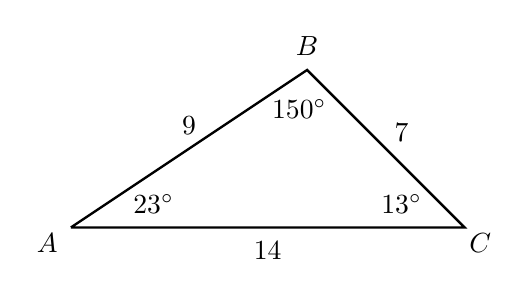
\begin{tikzpicture}
	\draw[line width=0.03cm] (0,0) -- (3,2) -- (5,0) -- (0,0);
	\node at (-0.3,-0.2) {$A$};
	\node at (3,2.3) {$B$};
	\node at (5.2,-0.2) {$C$};
	\node at (1.5,1.3) {$9$}; 
	\node at (4.2,1.2) {$7$}; 
	\node at (2.5,-0.3) {$14$}; 
	\node at (1.05,0.3) {$23^\circ$};
	\node at (4.2,0.3) {$13^\circ$};
	\node at (2.9,1.5) {$150^\circ$};
	\end{tikzpicture}
	\]
Find the following:
	\begin{enumerate}[(a)]
	\item $\angle FED$
	\item $|\overline{FD}|$
	\item $\angle EDF$
	\item $|\overline{DE}|$
	\item $\angle DFE$
	\item $\overline{EF}$
	\end{enumerate}



\newpage



% Problem 2
\problem{10} Does there exist a triangle with sides 5, 6, 12? If not, explain why. If so, construct. Do the same for a triangle with sides 5, 12, 13. 



\newpage



% Problem 3
\problem{10} A student is given a line segment $\overline{AB}$ and is told to construct the perpendicular bisector to the segment; that is, construct a line segment that is perpendicular to the given line segment that intersects the given line segment at a point $C$ such that $|\overline{AC}|= \overline{BC}|$. The student then performs the following:
	\begin{itemize}
	\item They draw a circle centered at $A$ with radius equal to the length of the line segment. 
	\item They draw another circle centered at $B$ with radius equal to the length of the line segment. 
	\item They find the two intersection points of the circles from the previous two steps and connect them.
	\end{itemize}
The student then claims that the final line segment drawn is the perpendicular bisector of the line segment $\overline{AB}$. Is the student correct? If so, prove that this is the perpendicular bisector. If not, explain what they have done incorrectly. 


\end{document}